% ! TeX root = *.tex
\documentclass{beamer}
\usepackage{copyrightbox}
\usepackage{graphicx}
\usepackage{xurl}
\graphicspath{{../img/}}
\setbeamertemplate{navigation symbols}{}
\usetheme{CambridgeUS}
\usecolortheme{seahorse}
\usepackage[german]{babel}
\usepackage[utf8]{inputenc}
\title[VWA-Präsentation]{Selective-Laser-Melting und Laser-Metal-Deposition im Vergleich}
\subtitle{Präsentation der Vorwissenschaftlichen Arbeit}
\author{Simon Wögerbauer}
\institute[Brucknergym Wels]{BG/BRG Wels Brucknerstraße\\
	Anton-Bruckner-Straße 16\\
	4600 Wels}
\date{16. April 2024}
\titlegraphic{
\includegraphics[scale=0.2]{brg_logo_2} \hspace*{.6\textwidth}
\includegraphics[scale=0.2]{brg_logo_2}} 
\makeatletter
\renewcommand{\CRB@setcopyrightfont}{%
\tiny
}
\makeatother
\makeatletter
\renewcommand{\CRB@setcopyrightparagraphstyle}{%
% Return to justifying text
\setlength{\rightskip}{0pt}
\setlength{\leftskip}{0pt}
}
\makeatother
\begin{document}
\frame{\titlepage}
% FOLIE 1
\begin{frame}
	\frametitle{\textit{Selective Laser Melting (SLM)}-Verfahren}

\begin{figure}
	\begin{centering}
	\copyrightbox[b]{
	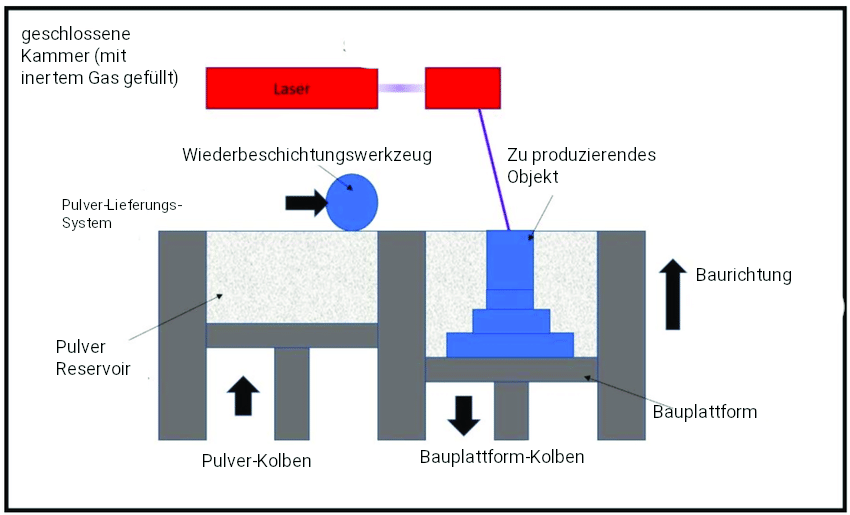
\includegraphics[width=.9\textwidth]{slm_diagram_edited.png}
}{\url{https://www.researchgate.net/publication/326891428/figure/fig1/AS:11431281211728231@1702484854583/Schematic-diagram-of-the-selective-laser-melting-SLM-process.tif}, bearbeitet durch den Autor}
	\end{centering}
\end{figure}
\end{frame}
\begin{frame}{Anwendungen}
\begin{figure}
	\begin{centering}
	\copyrightbox[b]{
	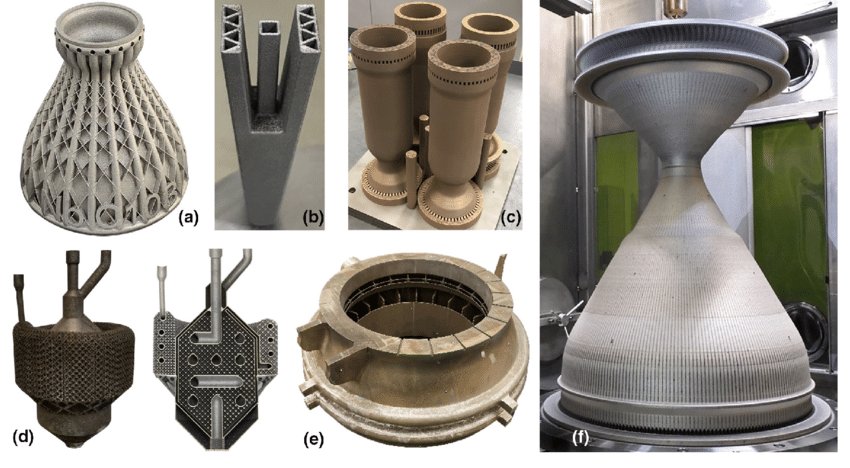
\includegraphics[width=.9\textwidth]{aero_2}
}{\url{https://www.researchgate.net/profile/Paul-Gradl/publication/360032150/figure/fig4/AS:1146451094708236@1650346649497/Examples-of-complex-aerospace-parts-fabricated-with-different-metals-and-alloys-a.png}}
	\end{centering}
\end{figure}
\end{frame}
\begin{frame}
\begin{figure}
	\begin{centering}
	\copyrightbox[b]{
	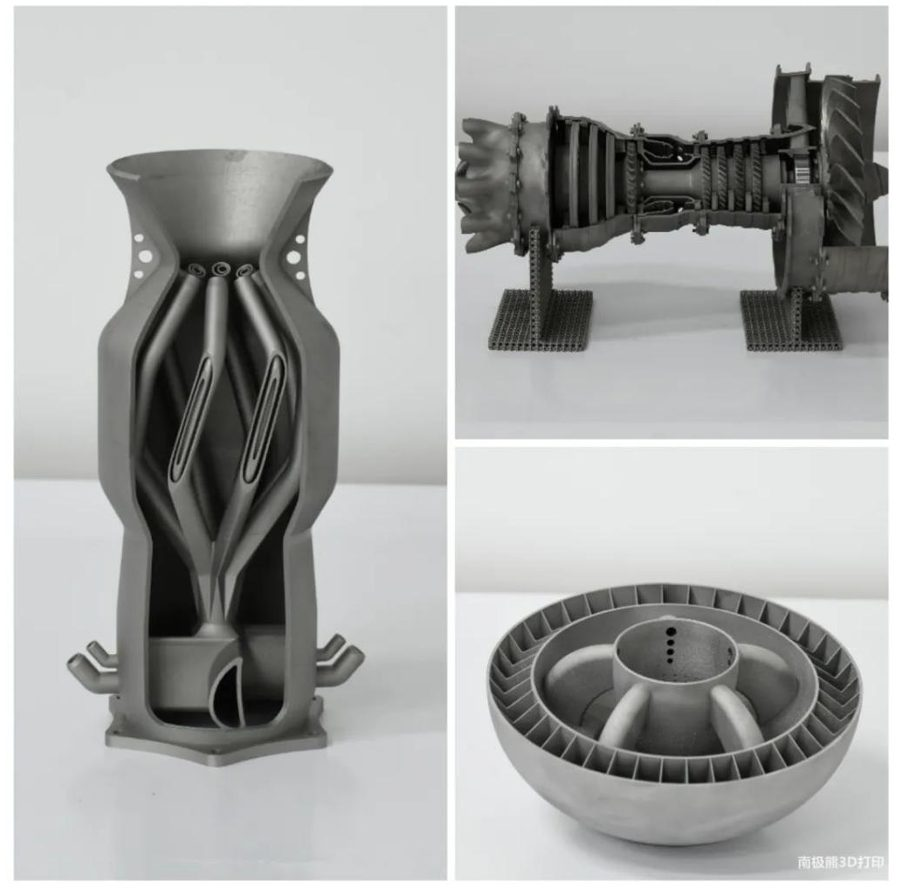
\includegraphics[width=.9\textheight]{aero_1}
}{\url{https://www.eplus3d.com/uploads/image/20220517/eplus3d-provides-large-metal-am-machines-to-jingye-additive-manufacturing-for-aerospace-1.jpg}}
	\end{centering}
\end{figure}

	
\end{frame}

\end{document}
